\section{Method}
\label{sec:method}

In this section, it is explained how the two subsystems are implemented and tested, using AIMSpice to create and test a 1-bit register, and Verilog to create the full circuit. 

\subsection{MAC design}
\label{subsec:circuitDesign}

This section specifically looks into how to implement the different subsystems of the MAC unit. The designs are shown at a logic gate level as that is used for both the AIMSpice and Verilog implementation. 

\subsubsection{Multiplier} 

A 2-bit multiplier could be designed like shown in \autoref{fig:multiplier}, which takes in A and B as two 2-bit inputs and outputs a 4-bit signal O. 

\begin{figure}[H]
    \centering
    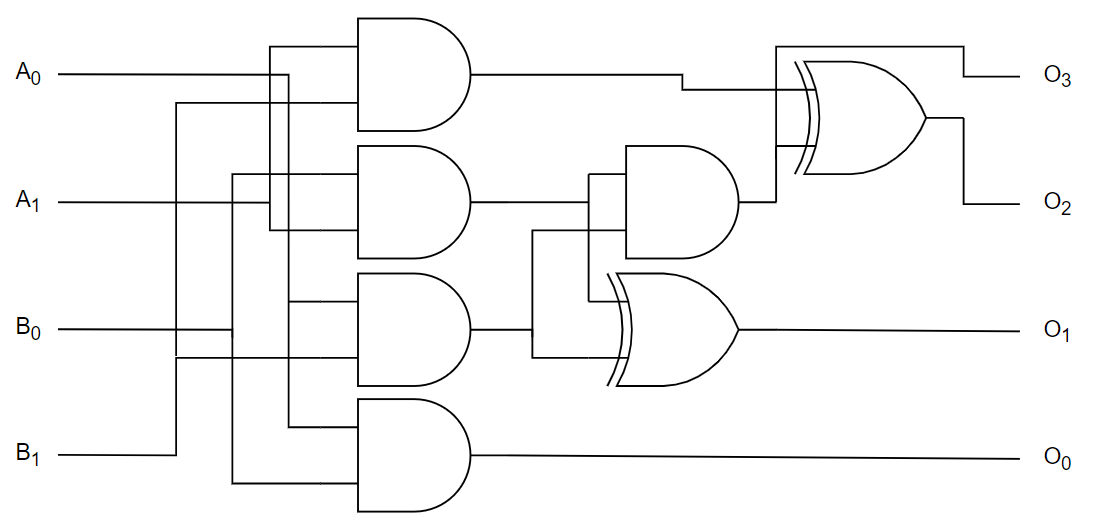
\includegraphics[width=0.8\textwidth]{Figures/multiplier.png}
    \caption{Possible design of a 2-bit multiplier.}
    \label{fig:multiplier}
\end{figure}

\subsubsection{Adder}

The design of an 8-bit adder is shown in \autoref{fig:adder-blokk}. The figure shows two 8-bit numbers A and B, and their sum S with a carry $C_O$. 

\begin{figure}[H]
    \centering
    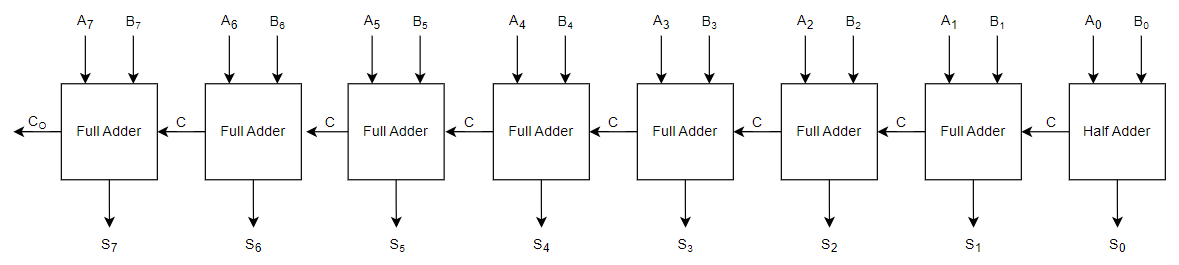
\includegraphics[width=\textwidth]{Figures/8bitadder.png}
    \caption{8-bit adder.}
    \label{fig:adder-blokk}
\end{figure}

The circuit for the half and full adder is shown in \autoref{fig:halfadder} and \ref{fig:fulladder}. 

\begin{figure}[H]
\begin{minipage}{0.4\textwidth}
    \centering
    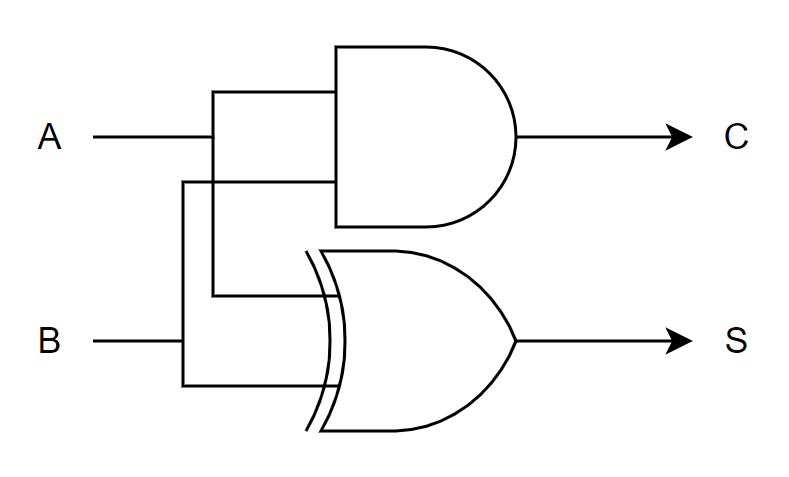
\includegraphics[width=\linewidth]{Figures/halfadder.png}
    \caption{Half adder.}
    \label{fig:halfadder}
\end{minipage}
\begin{minipage}{0.6\textwidth}
    \centering
    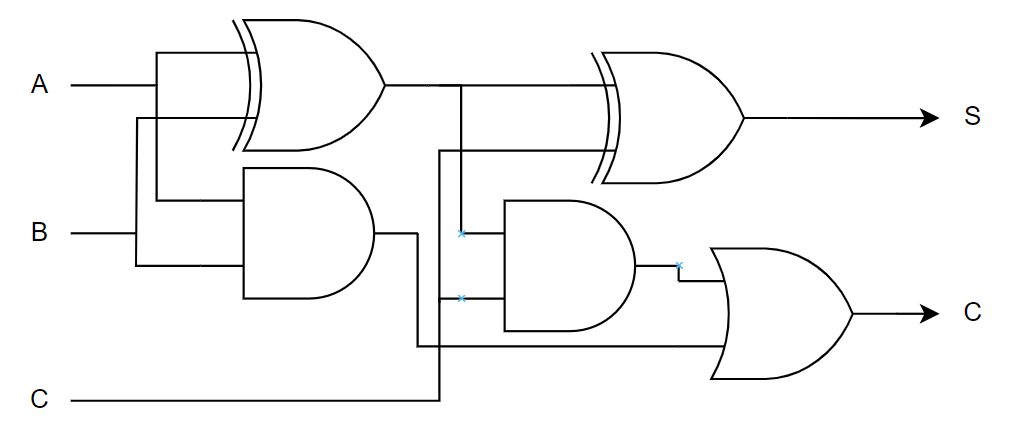
\includegraphics[width=\linewidth]{Figures/fulladder.png}
    \caption{Full adder.}
    \label{fig:fulladder}
\end{minipage}
\end{figure}


\subsubsection{Accumulator}
\label{subsubsec:accumulator}
The accumulator is an 8-bit register with some control signals, that is received from the FSM. 

\begin{figure}[H]
    \centering
    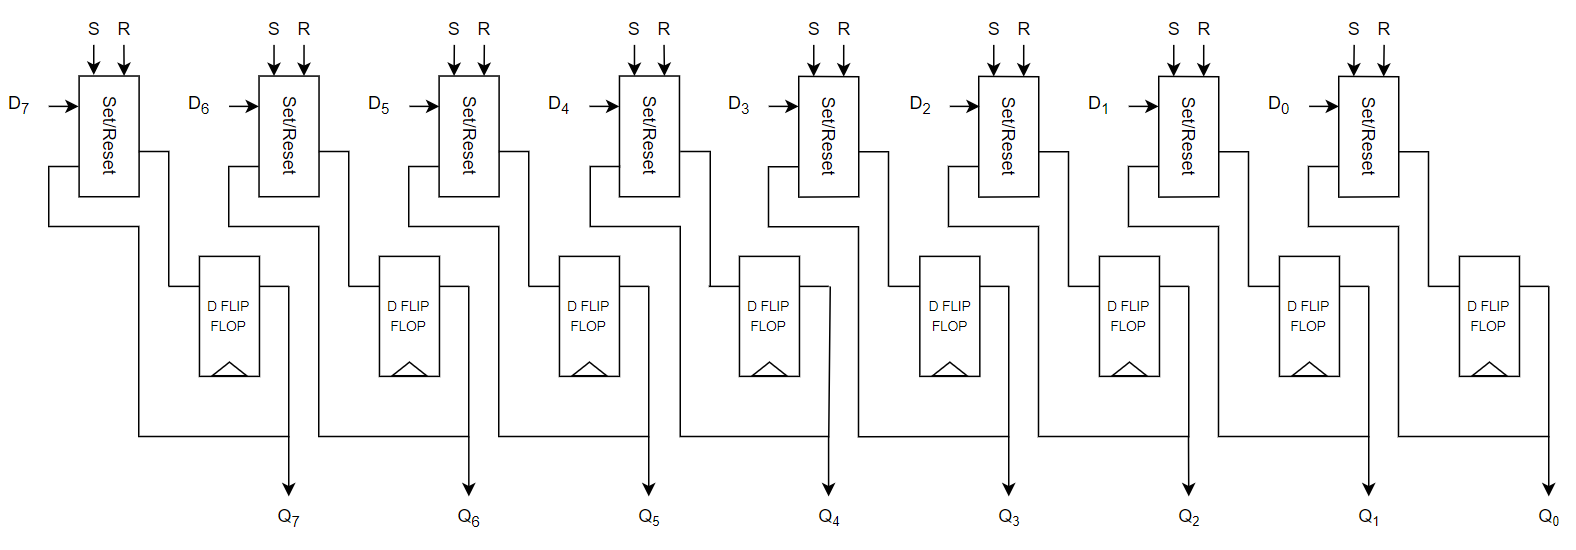
\includegraphics[width=0.9\textwidth]{Figures/8bitRegister.png}
    \caption{8-bit register.}
    \label{fig:8bitregister}
\end{figure}

As shown in \autoref{fig:8bitregister}, each bit of the accumulator consists of a D flip-flop and a control circuit. These are implemented as shown in \autoref{fig:dflipflop} \cite[p.18]{digital_design} and \ref{fig:setreset} respectively. This implementation of a D flip-flop gives a rising edge triggered D flip-flop. If the CLK signals were reversed at all transmission gates, the D flip-flop will become falling edge triggered.  

\begin{figure}[H]
    \centering
    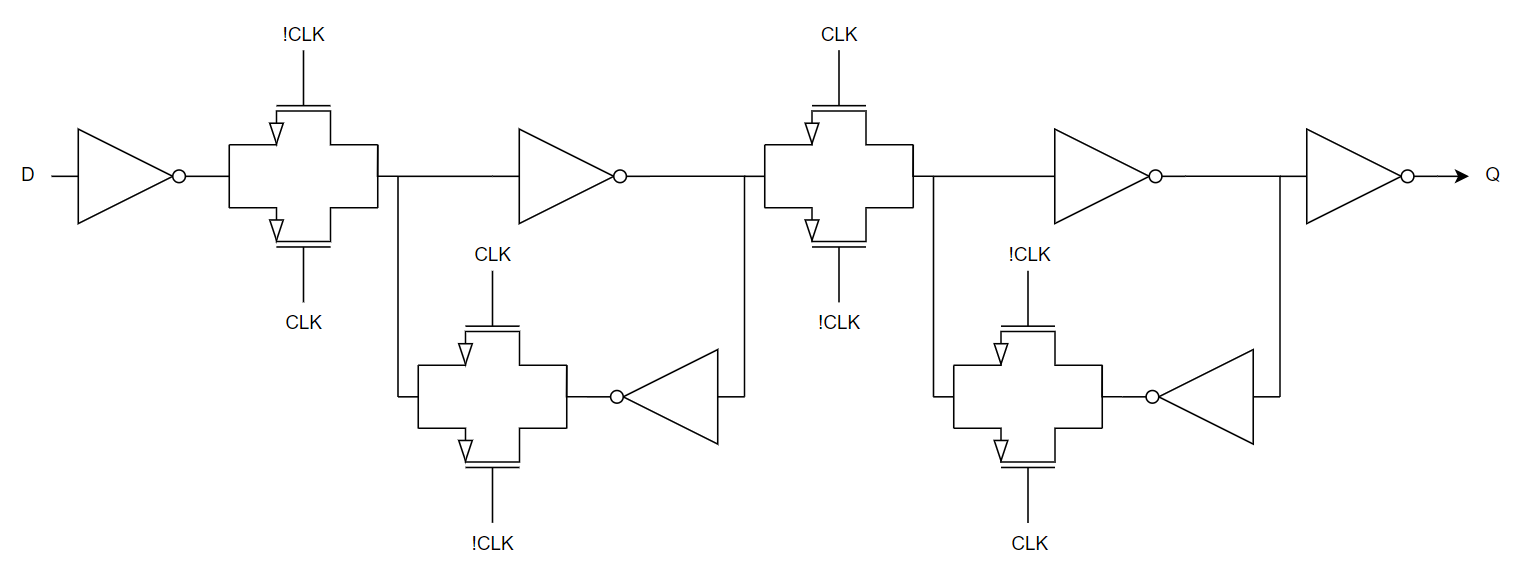
\includegraphics[width=\textwidth]{Figures/D_Flip_Flop.png}
    \caption{D flip-flop.}
    \label{fig:dflipflop}
\end{figure}

\begin{figure}[H]
    \centering
    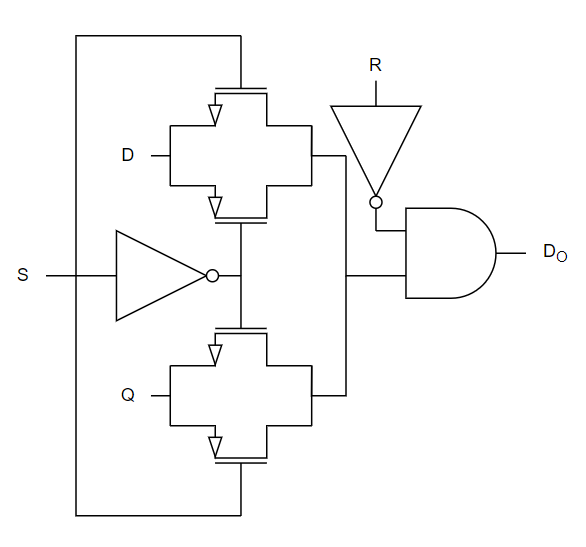
\includegraphics[width=0.4\textwidth]{Figures/setReset.png}
    \caption{Circuit for controlling register.}
    \label{fig:setreset}
\end{figure}

\subsection{FSM design}

The FSM was designed according to the project description and the design procedure given in \autoref{subsec:fsm_theory}. Both a Mealy and a Moore FSM design has been considered. The Mealy state machine resulted in four different states and the Moore machine resulted in eight different states, requiring an additional state register and more combinatorial logic. The final design was subsequently chosen to be a Mealy FSM, to minimize the amount of transistors. The state diagram derived from the text description is shown in \autoref{fig:fsm_diagram}. To be able to hold four different states, one pause state and three different run states, the FSM needs a 2-bit register with a reset function. 

\begin{figure}[H]
    \centering
    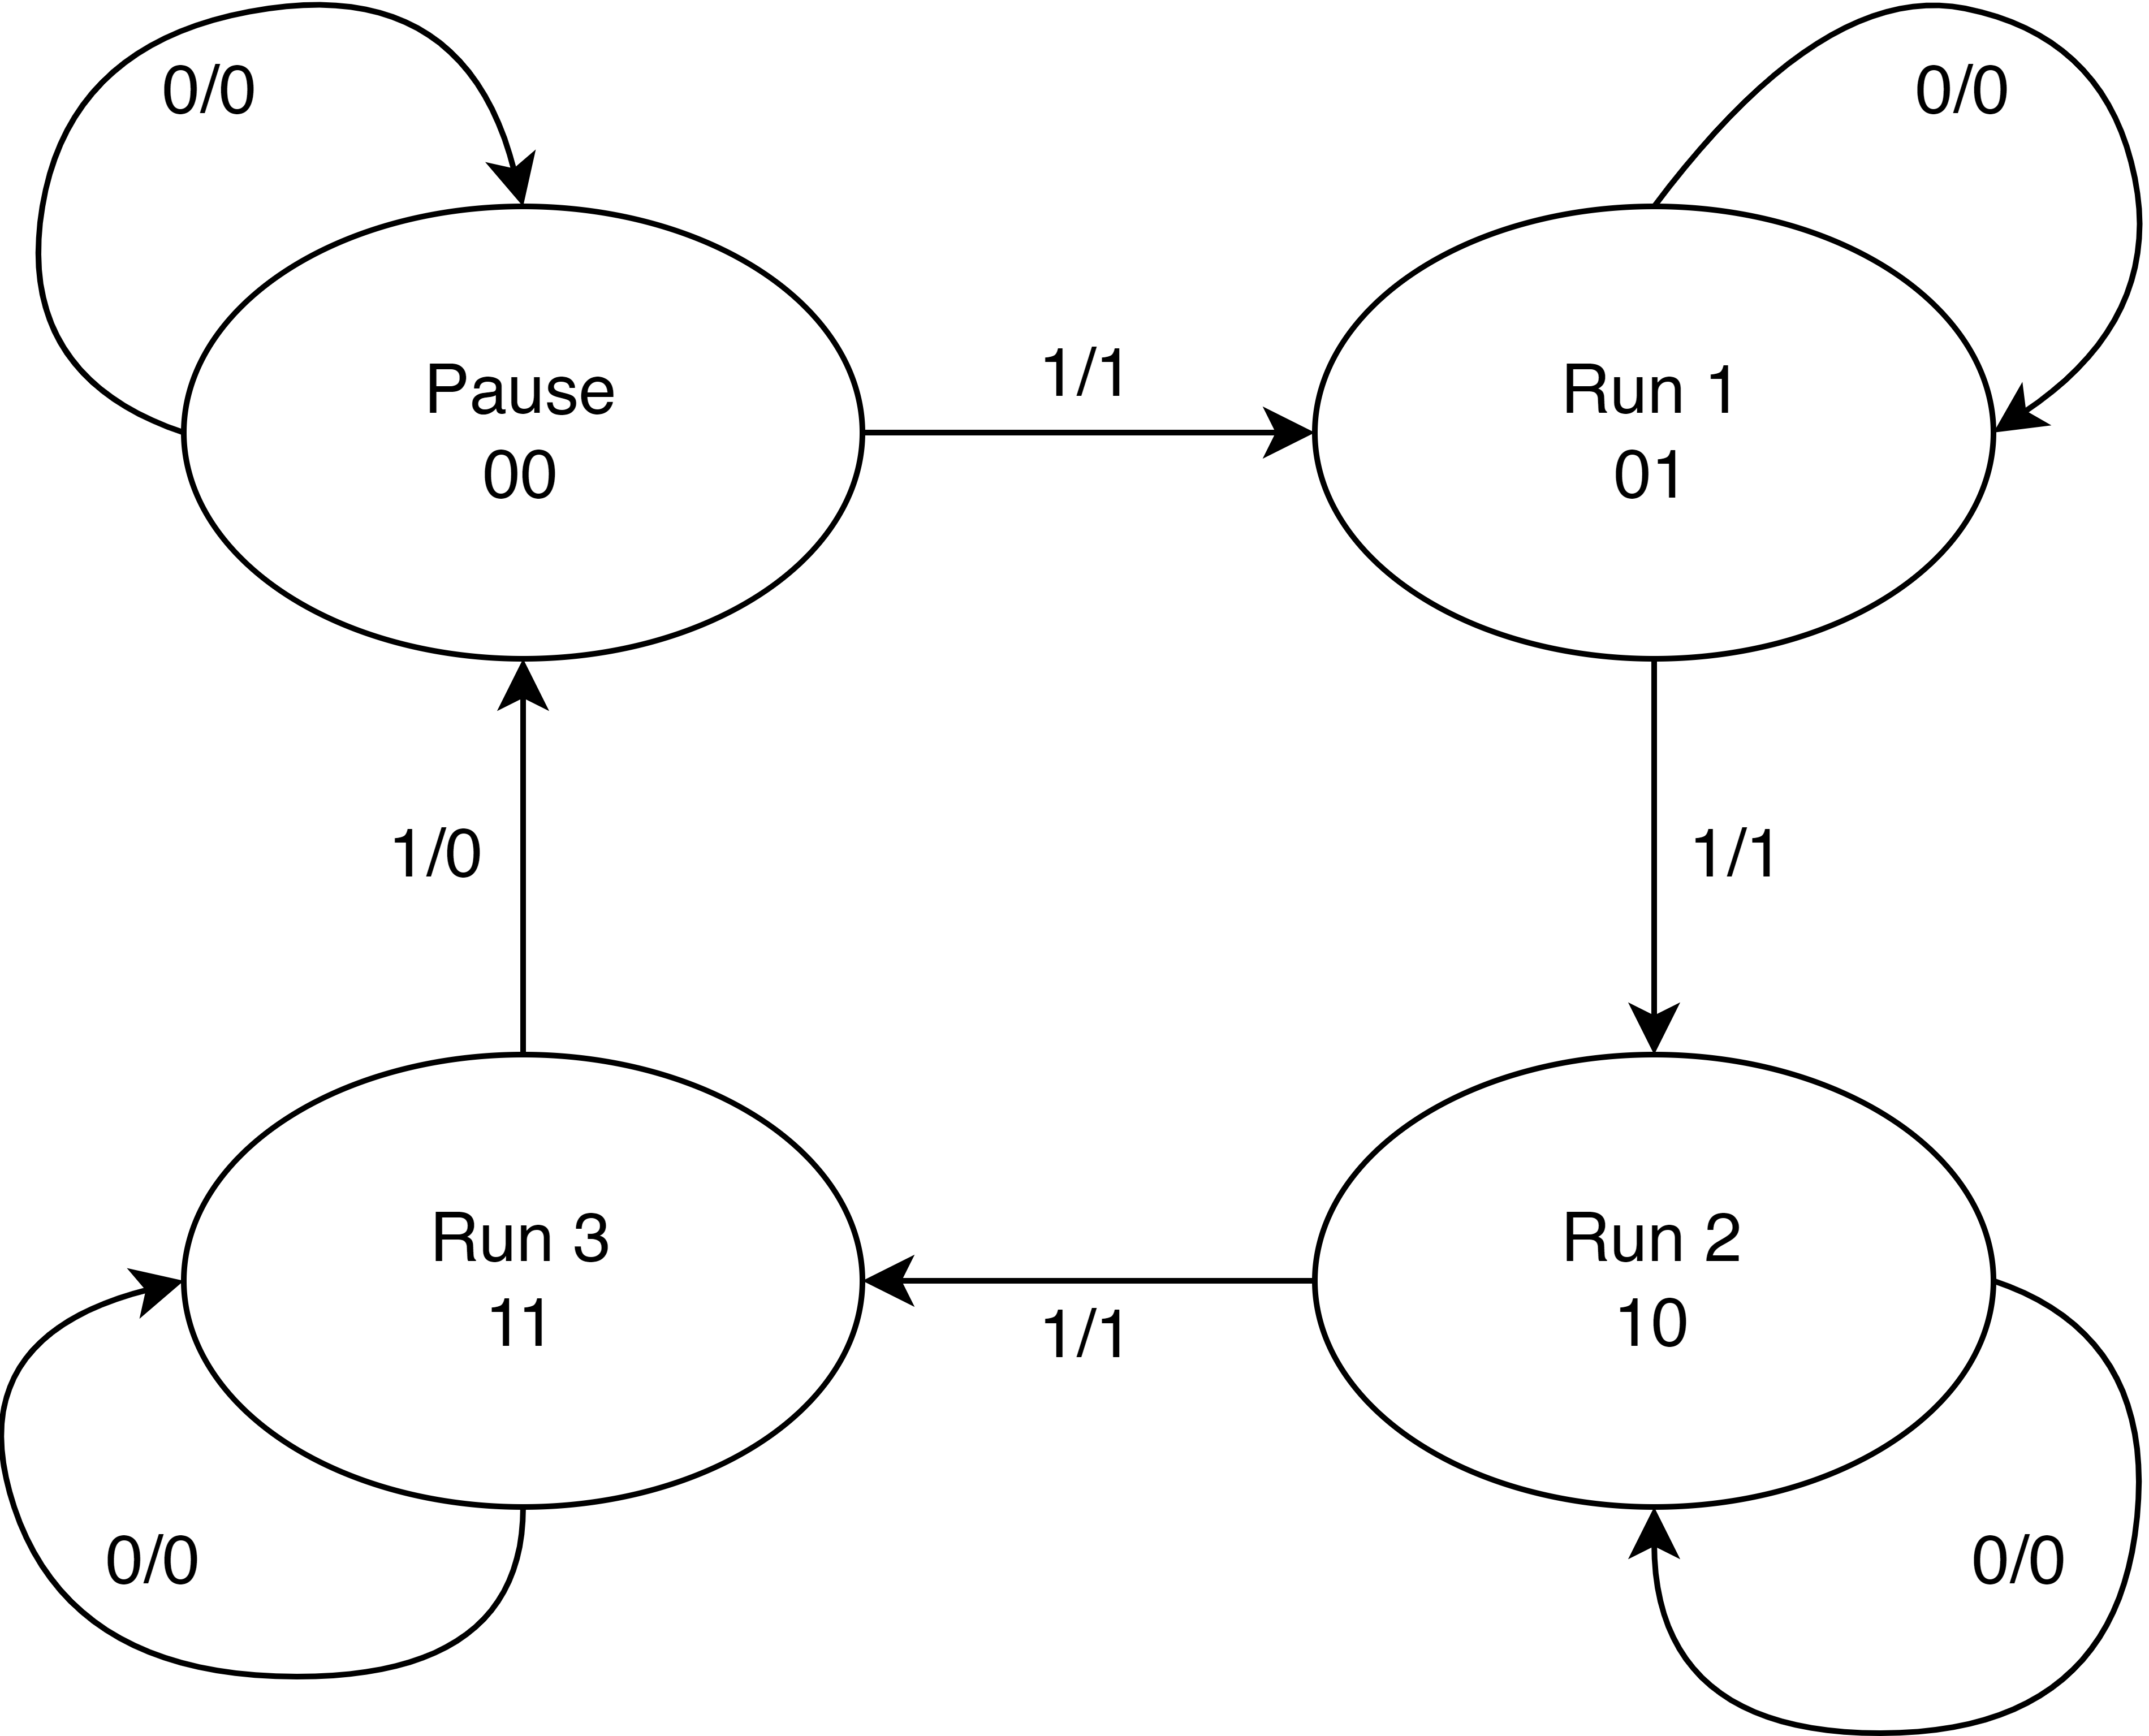
\includegraphics[width=0.8\textwidth]{Figures/FSM-diagram.png}
    \caption{FSM state diagram.}
    \label{fig:fsm_diagram}
\end{figure}

Three input signals are given by the specifications in \autoref{tab:specifications}, Reset, CLK and Run. The CLK signal
is only used to time the sequential logic in the FSM and passed on to the MAC unit without
further modification. The CLK signal is therefore not considered an input-signal here in the sense that it is not used in the next-state or output-logic in the FSM (see \autoref{fig:general_fsm}). The reset input signal $I_1$ is only used to reset the state register to the pause-state ``00'' and passed on to the MAC unit as $CTRL_1$ without further modification. The combinatorial part of the FSM is here only dependent on the current state ($C_1$ and $C_0$) and the Run input signal $I_0$. The outputs of the FSM are the next state signals $N_1$ and $N_0$, and the Reset and Run control signals $CTRL_1$ and $CTRL_0$. From the state diagram, we can write up the state table, \autoref{tab:state_table}. Note that $CTRL_1$ only is dependent on $I_1$ and that this does not require any gates.

\begin{table}[H]
\caption{State table for the FSM.}
\label{tab:state_table}
\centering
\begin{tabular}{|l|l|l|l|l|l||l|l|}
\hline
\rowcolor[HTML]{C0C0C0} 
$C_1$ & $C_0$ & $I_0$ & $N_1$ & $N_0$ & $CTRL_0$ & $I_1$ & $CTRL_1$\\
\hline
0  & 0  & 0  & 0   & 0   & 0 & 1 & 1\\ 
\hline
0  & 0  & 1  & 0   & 1   & 1 & 0 & 0\\ 
\hline
0  & 1  & 0  & 0   & 1   & 0 \\ 
\cline{1-6}
0  & 1  & 1  & 1   & 0   & 1 \\ 
\cline{1-6}
1  & 0  & 0  & 1   & 0   & 0 \\ 
\cline{1-6}
1  & 0  & 1  & 1   & 1   & 1 \\ 
\cline{1-6}
1  & 1  & 0  & 1   & 1   & 0 \\ 
\cline{1-6}
1  & 1  & 1  & 0   & 0   & 0 \\ 
\cline{1-6}

\end{tabular}
\end{table}

\noindent
The logic expression for each of the outputs of the combinatorial logic can be written down and simplified to \autoref{eq:comb_eq_1}, \ref{eq:comb_eq_2}, \ref{eq:comb_eq_3} and \ref{eq:comb_eq_4}.

\begin{equation}
\label{eq:comb_eq_1}
    CTRL_0 = I_0\cdot(\overline{C_1 \cdot C_0})
\end{equation}

\begin{equation}
\label{eq:comb_eq_2}
    N_0 = C_0 \oplus I_0
\end{equation}

\begin{equation}
\label{eq:comb_eq_3}
    N_1 = C_1 \oplus (C_0 \cdot I_0)
\end{equation}

\begin{equation}
\label{eq:comb_eq_4}
    CTRL_1 = I_1
\end{equation}

From the boolean equations, we can draw up the logic diagram, shown in \autoref{fig:fsm_logic_diagram}.

\begin{figure}[H]
    \centering
    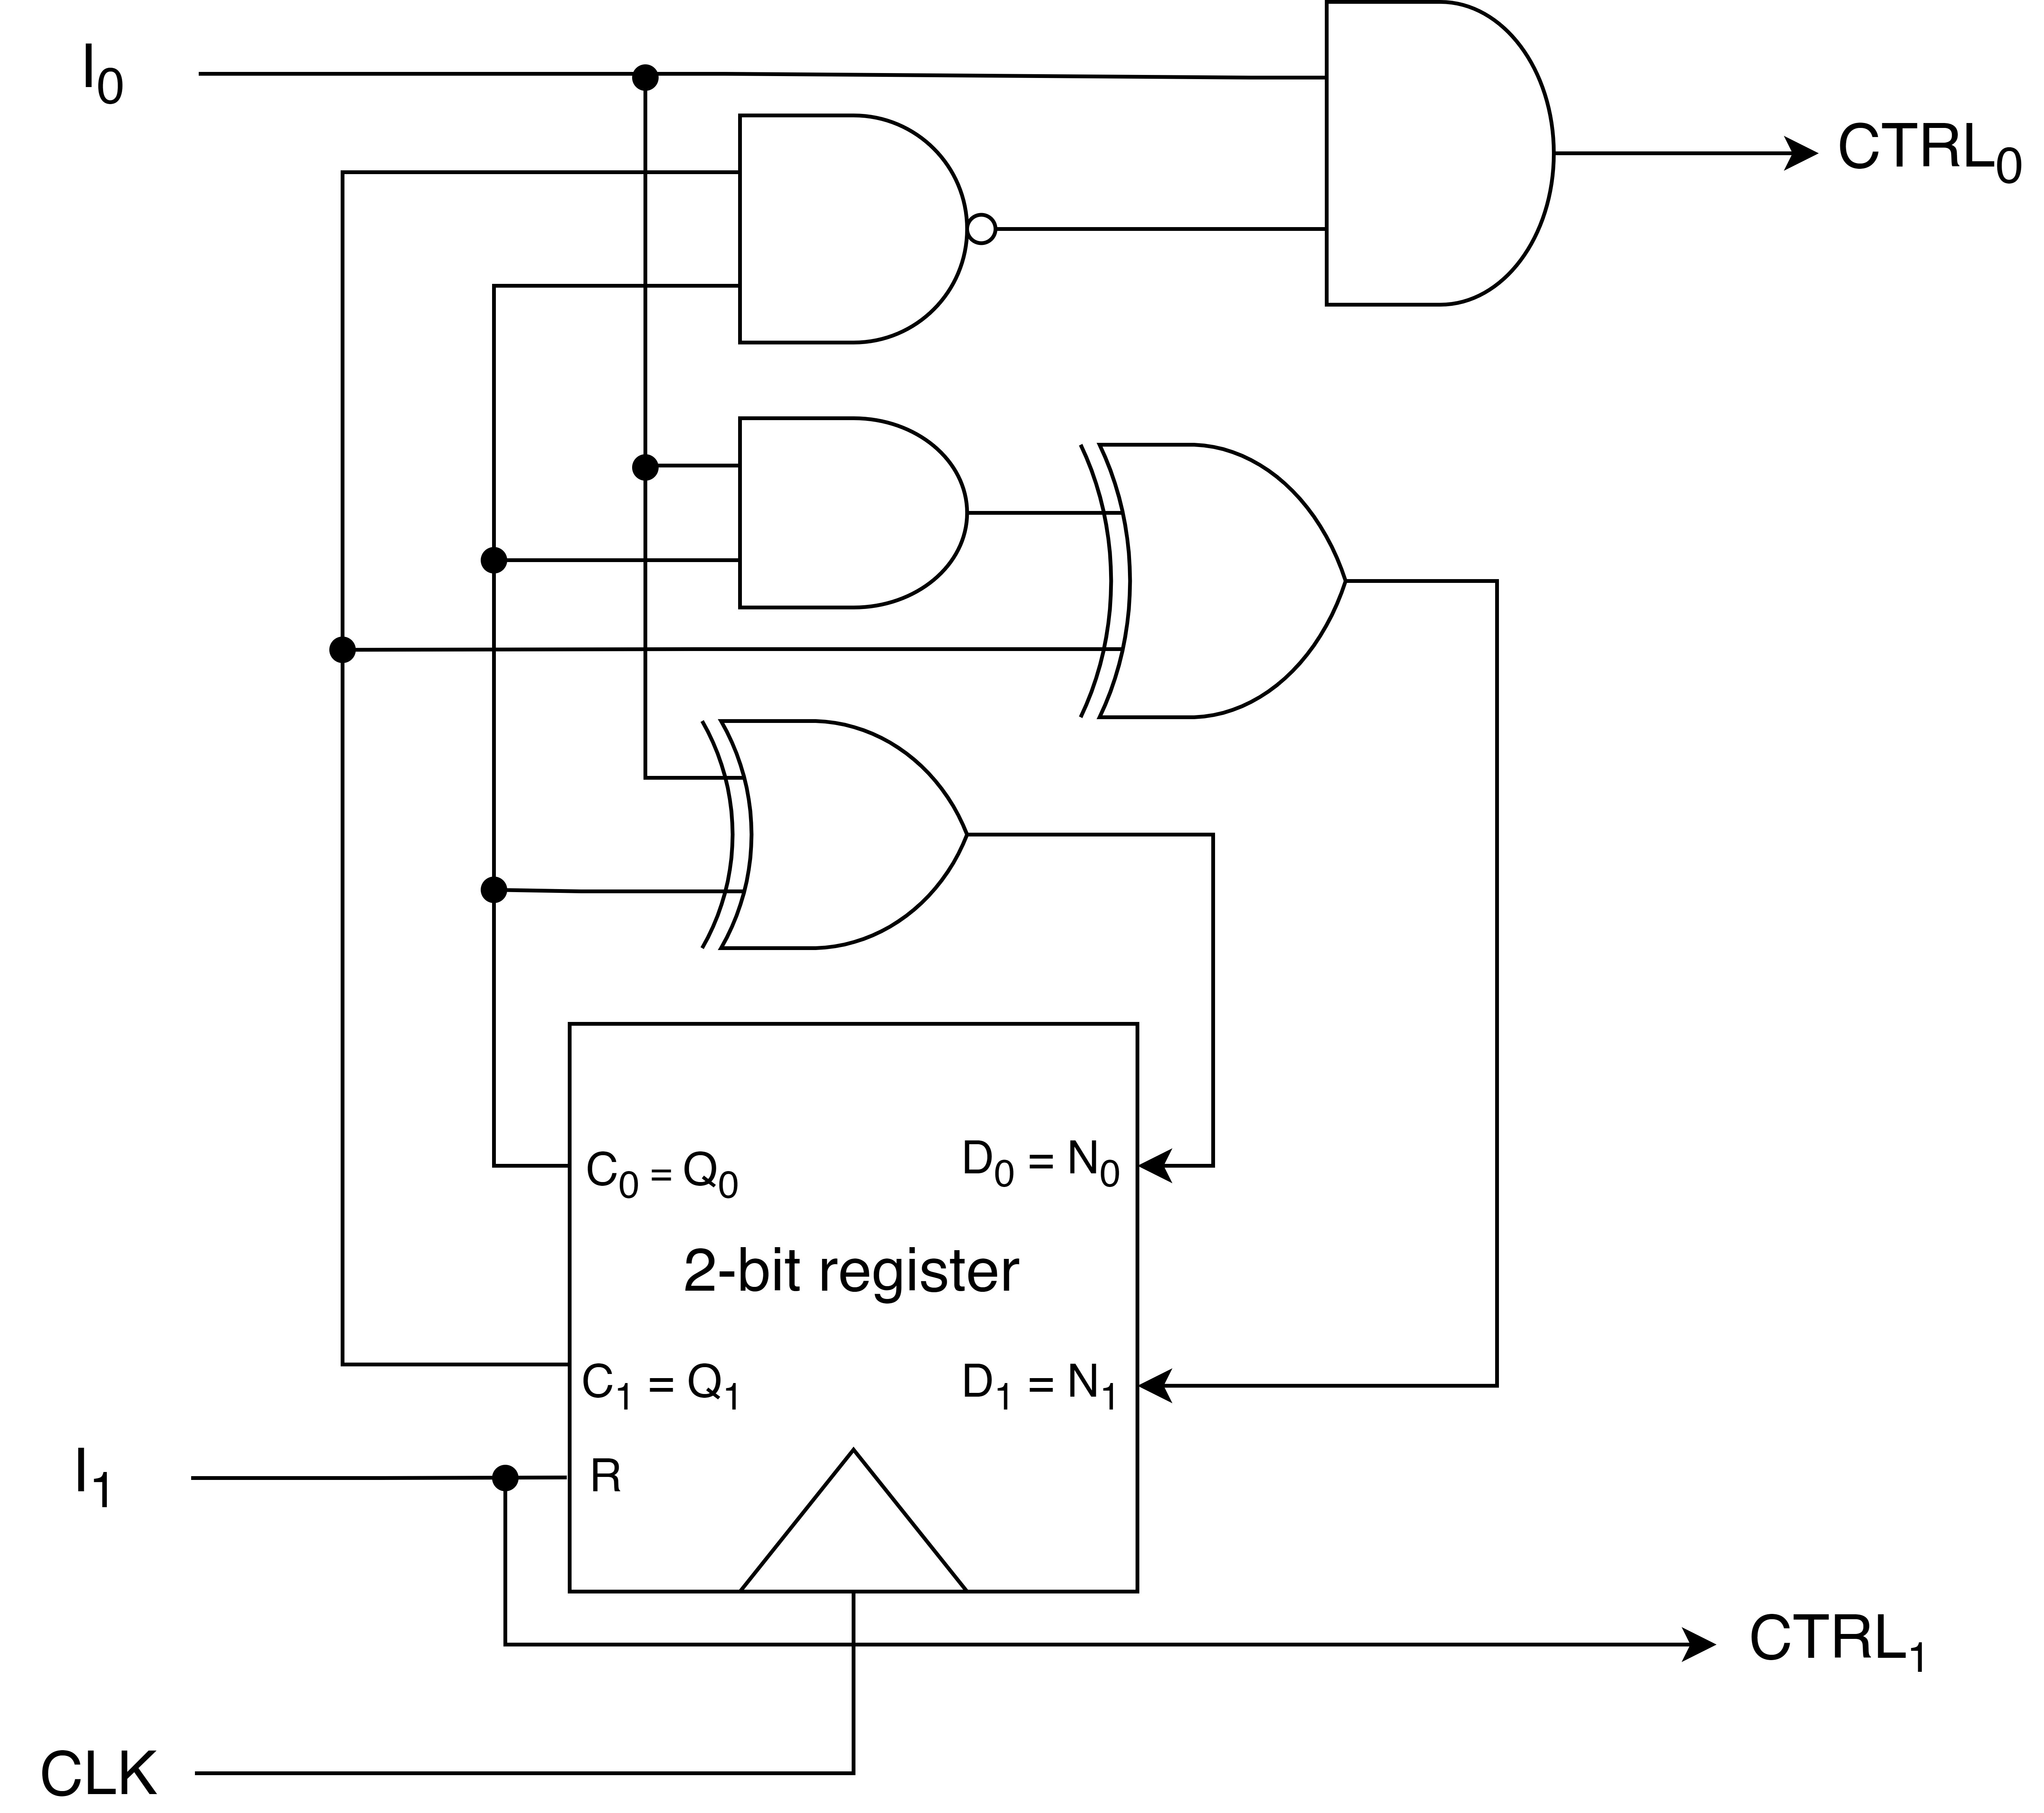
\includegraphics[width=0.6\textwidth]{Figures/logic diagram.png}
    \caption{FSM logic diagram.}
    \label{fig:fsm_logic_diagram}
\end{figure}

\noindent
The registers used in this circuit is of the same design as the register described in \autoref{subsubsec:accumulator}.

\subsection{AIMSpice}
\label{subsec:aimspicemethod}

In the AIMSpice related part of the assignment, a 1-bit register, \autoref{fig:1-bit_reg}, will be implemented using the designs shown in \autoref{fig:dflipflop} and \ref{fig:setreset}.

\begin{figure}[H]
    \centering
    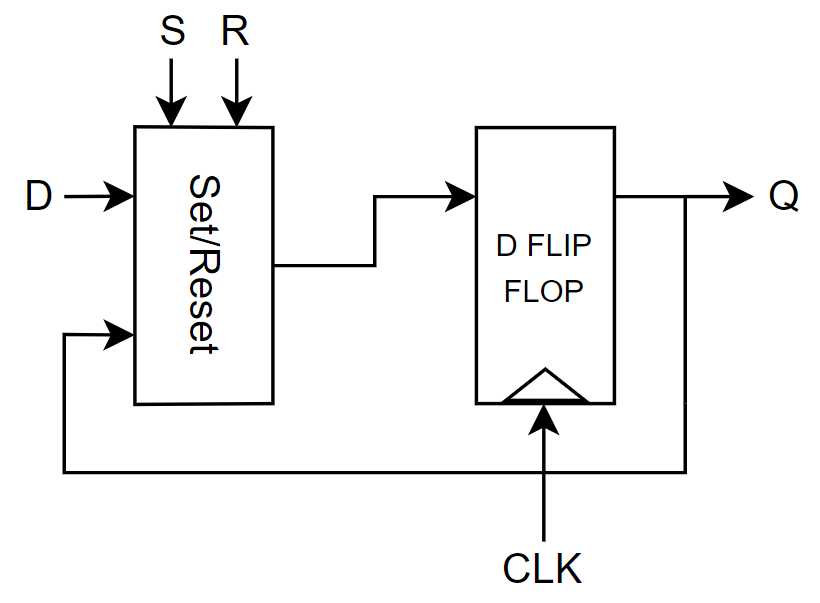
\includegraphics[width=0.6\textwidth]{Figures/1-bit register.png}
    \caption{1-bit register, with inputs Data, Reset and Set.}
    \label{fig:1-bit_reg}
\end{figure}

To implement the register in AIMSpice, different logic gates are made using transistors. The different logic gates used in the 1-bit register are NOT-, AND- and transmission gates. The transistor designs are shown in \autoref{fig:NOT}, \ref{fig:NAND}, \ref{fig:AND} and \ref{fig:TransGate}. To achieve a low static power consumption transistor stacking is used as that will give a lower leakage current. Through testing of different widths and lengths of the transistors, we found that a width of 100nm and a length of 300nm, gave the lowest leakage current while still having the correct functionality. 

\begin{figure}[H]
\centering
\begin{minipage}{0.4\textwidth}
    \centering
    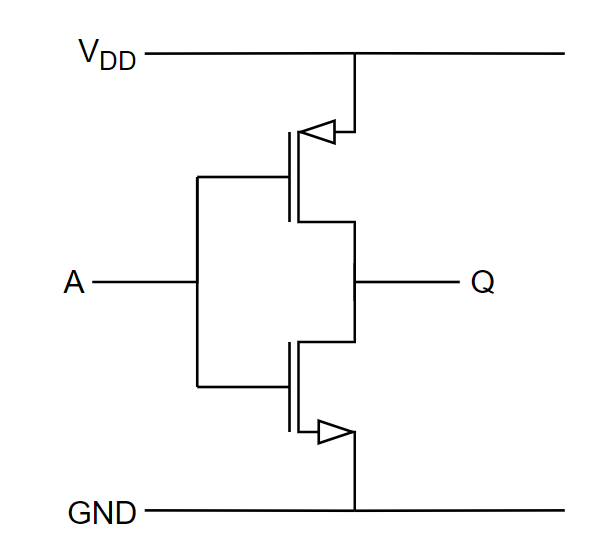
\includegraphics[width=\linewidth]{Figures/Not gate.png}
    \caption{\parbox{0.5\textwidth}{NOT-gate using MOSFET and transistor stacking.}}
    \label{fig:NOT}
\end{minipage}
\begin{minipage}{0.4\textwidth}
    \centering
    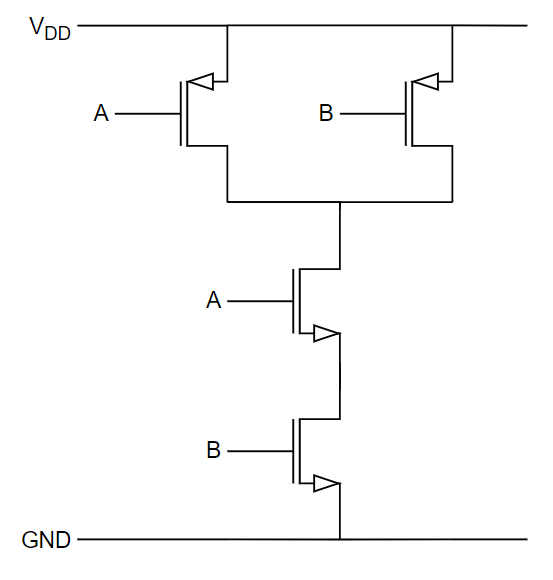
\includegraphics[width=0.9\linewidth]{Figures/Nand Gate.png}
    \caption{\parbox{0.5\textwidth}{NAND-gate using MOSFET and transistor stacking.}}
    \label{fig:NAND}
\end{minipage}
\end{figure}

The AND gate is made by connecting a NAND and NOT in series, as shown in \autoref{fig:AND}.
\begin{figure}[H]
    \centering
    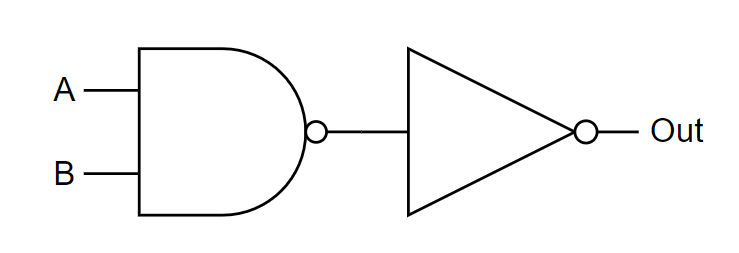
\includegraphics[width=0.4\linewidth]{Figures/And gate.png}
    \caption{AND gate.}
    \label{fig:AND}
\end{figure}

\begin{figure}[H]
    \centering
    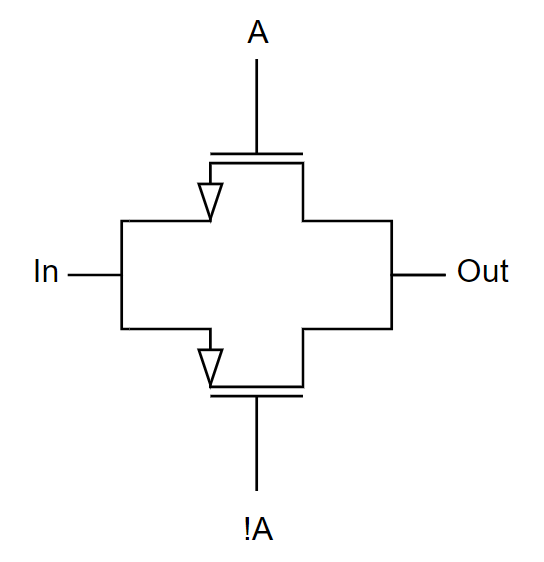
\includegraphics[width=0.4\linewidth]{Figures/Transmission gate.png}
    \caption{Transmission gate.}
    \label{fig:TransGate}
\end{figure}


\subsubsection{AIMSpice verification}
\label{subsubsec:aimspice_testing}
To test the 1-bit register made by in AIMSpice, we have to set some square waves for the clock signal, the data input, and the set and reset signals.

As shown in \autoref{fig:aimspice_pulses}, we use the PULSE function in AIMSpice to create square waves for the different inputs. These inputs will together determine what the output Q is set to.

\begin{figure}[H]
\centering
\begin{minipage}{0.9\textwidth}
\begin{lstlisting}[style=aimspiceStyle]
VD D 0 PULSE(0 C_VDD 25n RISE_TIME FALL_TIME 20ns 40ns)
VCLK CLK 0 PULSE(0 C_VDD 0 RISE_TIME FALL_TIME CLK_HIGH CLK_PERIOD)
VS S 0 PULSE(0 C_VDD 25n RISE_TIME FALL_TIME 60n 120n)
VR R 0 PULSE(0 C_VDD 145n RISE_TIME FALL_TIME 50n 100n)
\end{lstlisting}
\end{minipage}
\caption{AIMSpice code for creating square waves for the input signals, with all combinations of the inputs present.}
\label{fig:aimspice_pulses}
\end{figure}

The register should have the functionality as shown in the \autoref{tab:registerFunc}. Where the value of Q gets set to D if set is high and it keeps its previous value if set is low. If reset is high, the value Q is set to low. 

\begin{table}[H]
\centering
\caption{Functionality of 1-bit register}
\label{tab:registerFunc}
\begin{tabular}{|l|l|l|}
\cline{1-3}
\rowcolor[HTML]{C0C0C0} 
R & S & Q  \\ \cline{1-3}
0 & 0 & Q  \\ \cline{1-3}
0 & 1 & D  \\ \cline{1-3}
1 & 0 & 0  \\ \cline{1-3}
1 & 1 & 0  \\ \cline{1-3}
\end{tabular}
\end{table}


\subsection{Verilog}

In this section we create the subsystems and testbenches for them using the hardware descriptive language Verilog. A testbench for the full circuit is also created in this section.

\subsubsection{FSM in Verilog}
\label{subsec:fsm_verilog}

The FSM is implemented and its functionality is verified using Verilog. An excerpt of the logic part is given below in \autoref{fig:verilog_FSM_excerpt}. The complete code for implementing the FSM in Verilog is given in \autoref{verilog_FSM} in the appendix.


\begin{figure}[H]
\centering
\begin{minipage}{0.33\textwidth}
\begin{lstlisting}[style=verilogStyle]
xor(N[0], C[0], RunIN);
and(A, C[0], RunIN);
xor(N[1], A, C[1]);
nand(B, C[0], C[1]);
and(RunOUT, B, RunIN);
\end{lstlisting}
\end{minipage}
\caption{Excerpt of the FSM implemented in Verilog.}
\label{fig:verilog_FSM_excerpt}
\end{figure}


To simplify the implementation, the register is written as a separate module, shown in the appendix \autoref{verilog_onebitregister}.

To test the functionality, a separate testbench-module is made in verilog. The FSM is run through a series of different possible inputs. The output timing diagram is subsequently analyzed to verify that the FSM has the correct output based on the input.

\subsubsection{MAC in Verilog}
\label{subsubsec:MAC_in_verilog}

As the MAC is composed of three subcircuits, these are implemented, using the designs in \autoref{subsec:circuitDesign}, and tested with Verilog testbenches separately. All the code for the implementation of the subsystems are found in \autoref{appendix:Verilog-code}. 

The 2-bit multiplier and the 8-bit adder is set up to loop through all possible combinations of inputs and checked if the output matches what is expected. \autoref{fig:verilog_adderTB_excerpt} shows how to loop through the inputs on the adder.

\begin{figure}[H]
\centering
\begin{minipage}{0.8\textwidth}
\begin{lstlisting}[style=verilogStyle]
for(Acount = 0 ; Acount < 256 ; Acount++) begin
    for(Bcount = 0 ; Bcount < 256 ; Bcount++) begin
        A = Acount;
        B = Bcount;
        #1;
        if((A+B) == S) begin
            $display(A,"+",B,"=",S);
        end else begin
            $display("Error: ", A, "+", B, "=",S);
            errors++;
        end
    end
end
\end{lstlisting}
\end{minipage}
\caption{Loop to check all combinations for the adder.}
\label{fig:verilog_adderTB_excerpt}
\end{figure}

A and B are 8-bit input signals to the adder which can represent unsigned integers 0 to 255. Note the small delay needed for the signals to propagate the circuit. A similar approach can be used to verify the functionality of the multiplier and the register. 

For the register testbench, given in \autoref{verilog_registerTB}, one also has to account for the delay needed for the clock to have one rising edge before next input is tested. A testbench was also made for the MAC put together without the FSM. The procedure used for this testbench is the same as described in \autoref{subsubsec_FullMAC_verilog}. All testbenches can be found in \autoref{sec:verilog_testbenches}.

\subsubsection{Full MAC in Verilog}
\label{subsubsec_FullMAC_verilog}

Finally, to test the entire MAC put together the modules are put together as a complete circuit, shown in \autoref{verilog_fullmac}. A testbench is created to empirically test different combinations of inputs. As all combinations of current and previous inputs cannot easily be tested, like for the adder and multiplier isolated, the complete circuit is put through a series of randomized inputs A and B using the system function ``\$random''. The simulation can be repeated for different inputs by changing the variable ''randomSeed'' to a different integer.

% \subsection{Must include}
% The method section MUST INCLUDE:
% \begin{itemize}
%     \item One or more illustrations showing your circuit. As a minimum you must include one figure of the circuit at the logic gate level, and one of what you implemented at transistor level in AIMSpice.
%     \item Figure showing the state diagram for your final state machine (FSM).
%     \item Explanations of design choices you made when creating the circuit.
%     \item Explanations of the simulations you did (not the results, just how they were done).
% \end{itemize}